\documentclass[12pt,a4paper, oneside]{article}
\usepackage[utf8]{inputenc}
\usepackage[T1]{fontenc}
\usepackage[english,german]{babel}
\usepackage[style=german]{csquotes}
\usepackage{graphicx}

\author{Uni Oldenburg, SWP2020 Gruppe A}

\begin{document}

    \begin{titlepage}
        \pagestyle{empty}
        \begin{center}

            \begin{figure}[h]
                \centering
                
\includegraphics[width=0.35\textwidth]{img/Logo.jpg}
            \end{figure}

            \bigskip \bigskip \noindent
            \textsc{\textbf{\LARGE Softwareprojekt:}} \par \bigskip \noindent
            \textsc{\textbf{\LARGE Projekttagebuch}}


            \par \bigskip \bigskip \bigskip \bigskip \bigskip \noindent
            {\Large Gruppe A} \par \medskip \noindent

            \par \bigskip \bigskip \bigskip \bigskip \bigskip \bigskip \noindent
            \textit{\Large Wintersemester 2020/21 und} \par \noindent
            \textit{\Large Sommersemester 2021}

            \par \bigskip \bigskip \bigskip \bigskip \bigskip \bigskip \noindent
            \par \bigskip \bigskip \bigskip \noindent
            {\Large Sprintanalyse} \par \medskip \noindent

        \end{center}
    \end{titlepage}

    \tableofcontents
    \pagebreak


    \section{Sprinttagebuch: Sprint-Nr.4}
    \underline{Name des Sprints:}
    \\
    A New Hope

    \noindent
    \\
    \underline{Zeitraum des Sprints:}
    \\
    14. Januar 2021 bis zum 2. Februar 2021

    \noindent
    \\
    \underline{Ziel des Sprints:}
    \\
    Grundstruktur für Spielumsetzung

    \noindent
    \\
    \underline {Team:}
    \\
    Sven Ahrens, Alwin Bossert, Aldin Dervisi, Marvin Drees, Mario Fokken,
    Timo Gerken, Finn Haase, Temmo Junkhoff, Maximilian Lindner, Steven Luong,
    Phillip-André Suhr, Eric Vuong


    \section{Vorgänge}
    \begin{itemize}
        \item SWP2020A-37: ANmi, dass eine Partie von einer Lobby aus gestartet wird, sobald alle Lobbymitglieder sich bereiterklärt haben, damit alle an der Partie teilnehmen können. (9 Story Points)
        \item SWP2020A-41: UserManagement durch relationale Datenbank. (11 Story Points)
        \item SWP2020A-97: In Tests lock.await(1000, TimeUnit.MILLISECONDS) reduzieren. (2 Story Points)
        \item SWP2020A-98: Versteckte IDs in Listviews einbauen für bessere Eindeutigkeit, z.B. in ChatView. (4 Story Points)
        \item SWP2020A-99: Namenskonventionen für @Subscribe- \& ButtonPressed-Methoden erstellen und anwenden. (3 Story Points)
        \item SWP2020A-101: Lobby-Chathistorie bleibt nach Löschen einer Lobby erhalten. (2 Story Points)
        \item SWP2020A-102: Ausloggen schließt Lobbys nicht. (3 Story Points)
        \item SWP2020A-103: ANmi ein Spielfeld sehen, das den aktuellen Spielstand darstellt. (8 Story Points)
        \item SWP2020A-104: ANmi ein grundlegendes Zugsystem haben, sodass immer nur ein Spieler mit dem Spiel interagieren kann. (7 Story Points)
        \item SWP2020A-105: ANmi meine Ressourcen/Eigenschaften sehen können. (4 Story Points)
        \item SWP2020A-111: ANmi, dass der aktuelle Spielstand gespeichert wird und verfügbar ist. (8 Story Points)
        \item SWP2020A-149: Codestyle überarbeiten \& frisch anwenden. (2 Story Points)
    \end{itemize}

    \subsection{Sprinterfolg}
    \begin{figure}[h]
        \centering
        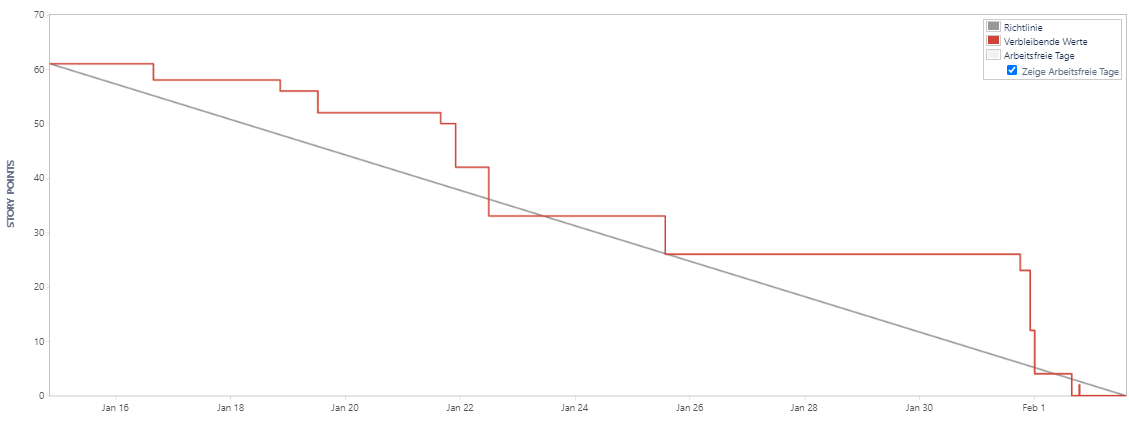
\includegraphics[width=\textwidth, height=5cm]{img/sprint_04/Burndown Sprint 4.png}
        \caption{Burndown-Diagramm Sprint 4}
        \label{fig: Burndown-Diagramm Sprint 4}
    \end{figure}
    Bei unserem Sprintbeginn hatten wir 61 offene Story Points. In unserem Burndown-Diagramm ist gut zu sehen, dass wir aus unseren Retrospektiven zuvor gelernt haben. Wir haben uns nämlich vorgenommen, dass wir bereits in der ersten Woche unseres Sprints einige unserer User Stories abschließen. Demnach hatten wir bei diesem Sprint bereits am 16. Januar die erste User Story (SWP2020A-99) abgearbeitet. Bei der Hälfte des Sprints waren bereits 6 User Stories fertig, sodass wir noch bei einem Sprintumfang 33 Story Points waren. Demnach haben wir das oben genannte Ziel der Retrospektive erfüllt. Außerdem kann man gut erkennen, dass wir uns nah an der vorgesehenen Richtlinie des Burndown-Diagramms bewegt haben. In der letzten Woche des Sprints haben wir uns zuerst etwas von der Richtlinie distanziert, am Ende dann jedoch alle User Stories abgeschlossen. Besonders auffällig ist der 1. Februar, da dort eine User Story unserem Sprint hinzugefügt wurde (SWP2020A-149). In dieses Story wurde der gesamte Code-Style im Projekt angepasst. Sinnvollerweise wurde dies am Ende des Sprint durchgeführt. Nachdem auch diese User Story beendet wurde, waren wir am 1. Februar mit allen User Stories fertig. Demnach hatten wir nach Sprintabschluss keine offenen User Stories, sodass unser nächster Sprint mit neuen Aufgaben starten konnte.

    \subsection{Sprintprobleme bzw. Hindernisse}
    Folgende Bugs und Verbesserungsmöglichkeiten sind uns im Sprint aufgefallen und sollten im nächsten Sprint bearbeitet werden:

    \begin{itemize}
        \item SWP2020A-115: SecurityException bei nicht eingeloggten Clients bei Lobbyerstellung
        \item SWP2020A-121: @Injects konkretisieren und korrigieren
        \item SWP2020A-122: Fenster sollen Mindestdimensionierung bekommen
        \item SWP2020A-150: StartSession-Button ist nach dem Start einer Session immer noch anklickbar
    \end{itemize}


    \section{Erkenntnis aus der Retrospektive}
    Folgende Action-items konnten wir für die Zukunft schließen:\\

    Was lief gut?
    \begin{itemize}
        \item Weiterhin um Hilfe bitten und Hilfe so oft es geht anbieten
        \item Pair-Programming beibehalten
        \item Weiter bereits in der ersten Woche an Vorgängen arbeiten
        \\
    \end{itemize}

    Was lief nicht so gut?
    \begin{itemize}
        \item Versucht alles kaputt zu machen in den Tests, denn was schiefgehen kann, wird auch schiefgehen
        \item Edgecases bei Tasks beachten
        \\
    \end{itemize}

    Was sollte anders laufen?
    \begin{itemize}
        \item Mehr Zeit nehmen, um Reviews ausführlicher durchzuführen
        \item Praxis Tests (Bei Review die hinzugefügten Features auch ausprobieren)
        \item Beim Reviewen auf die Tests achten (Anzahl und Edge-Cases)
        \item Sprint erweitern, falls einige ohne Arbeit sind
        \item Der frühere Vogel fängt noch mehr (So früh wie möglich mit Bearbeitung starten)
    \end{itemize}


    \section{Sonstige Anmerkungen}
    Ab dem folgenden Sprint werden wir deutlich mehr dokumentieren. Das beinhaltet die Dokumentation im Confluence, dieses Tagebuch und Dokumentation im Quellcode.
    Des Weiteren wurde abgesprochen, dass Commit-Messages in Zukunft präziser formuliert werden. Diese beinhalten nun einen aussagekräftigen Titel und anschließend eine Beschreibung jeglicher Änderungen in diesem Commit. Dadurch sollen beispielsweise Code-Änderungen für Reviewer leichter zu verstehen sein.


    \section{Fazit}
    Insgesamt war dieser Sprint sehr erfolgreich, da sowohl alle User Storys bearbeitet wurden, als auch der Umfang des Sprint deutlich höher war als der vorherige Weihnachts-Sprint. Die Bearbeitung der einzelnen Tasks beginnt nun deutlich früher als vorher, sodass wir uns gut an der Richtlinie des Burndown-Diagramms lang arbeiten konnten, wobei hier trotzdem noch Luft nach oben ist. Ab dem nächsten Sprint wird ein verstärktes Augenmerk auf die Reviews gelegt, damit weniger Bugs auftreten und wir uns weiter auf die Umsetzung der tieferen Spiellogik konzentrieren können. Außerdem werden wir in den zukünftigen Meetings nachfragen, ob jeder genug zu tun hat, um gegebenenfalls den Sprint zu erweitern.
\end{document}